%Leer en detalle y resumir en 6–8 viñetas: problema de la termalización, idea central de ETH, por qué el caos importa.
%1 slide de “mapa mental” + glosario de 10 términos.
\begin{frame}
\frametitle{ETH?}
\begin{figure}
    \centering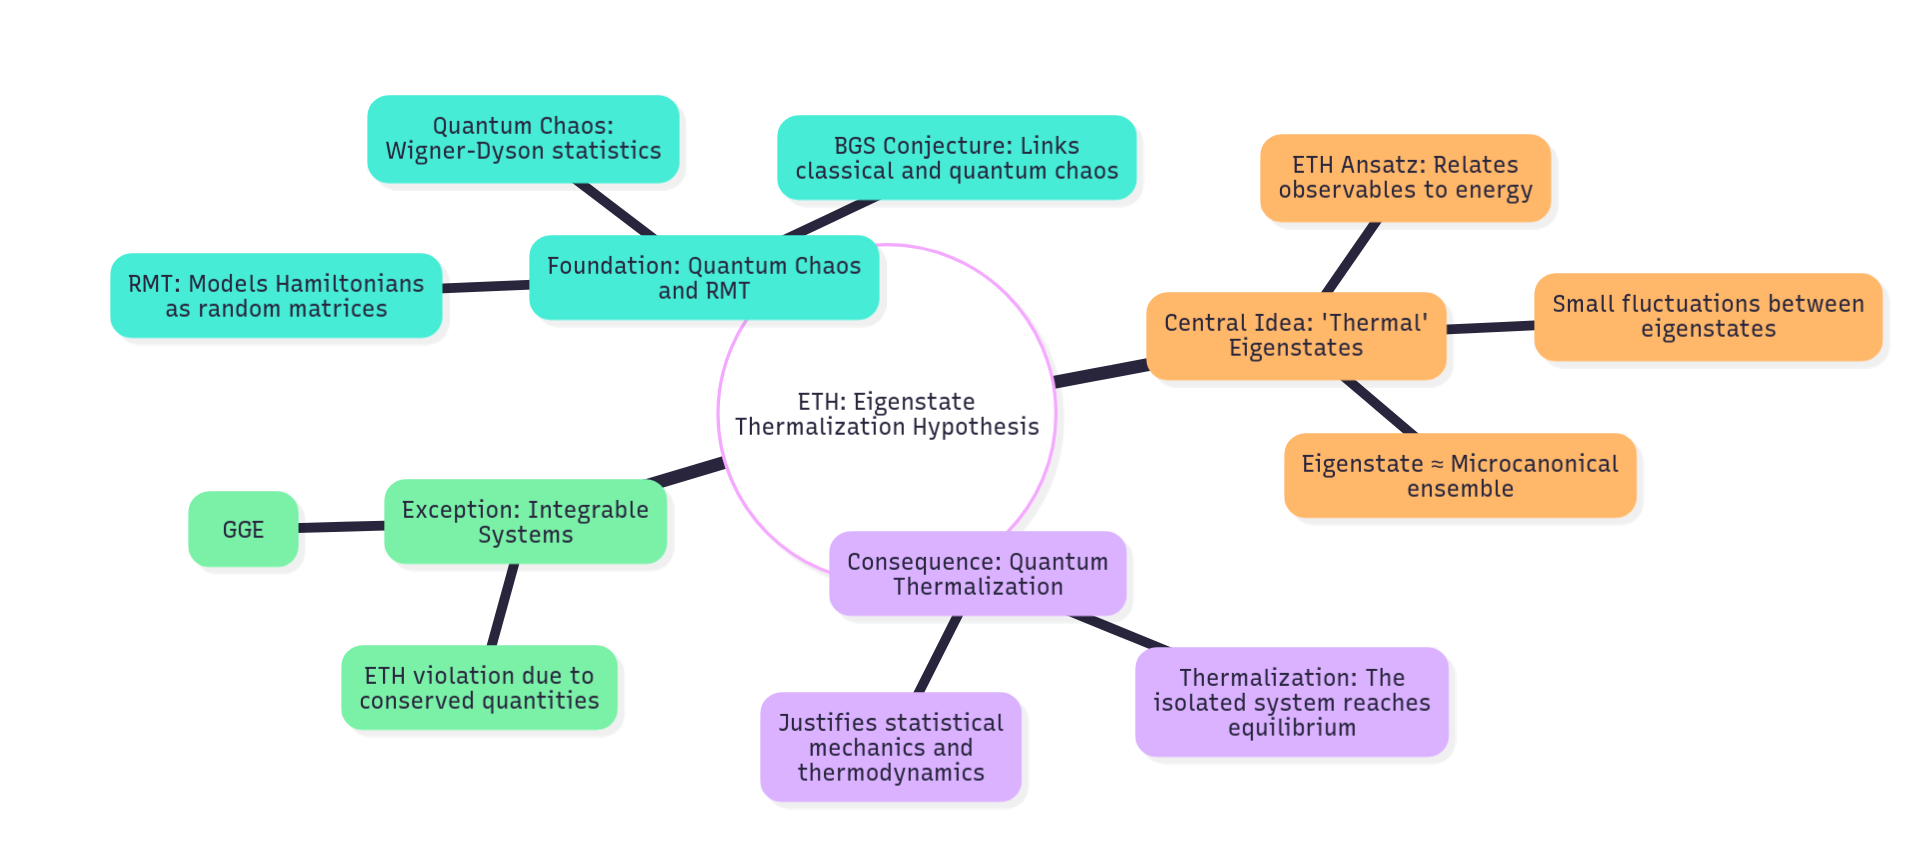
\includegraphics[width=\textwidth]{images/mindmap-ETH.png}
    \label{fig:ETH}
\end{figure}
\end{frame}

\begin{frame}
    \frametitle{Key Concepts in Quantum Thermalization}
    \framesubtitle{Fundamental Terms of Chaos and Equilibrium in Quantum Systems}

    \vspace{0.5cm}

    % --- Two-column layout ---
    \begin{columns}[T,onlytextwidth] % Align columns at the top

        % --- Left Column ---
        \begin{column}{0.48\textwidth}
            \begin{block}{Phenomena and Processes}
                \begin{itemize}
                    \item Thermalization
                    \item Quantum Chaos
                    \item Quantum Quench
                    \item Prethermalization
                    \item Delocalization
                \end{itemize}
            \end{block}
        \end{column}

        % --- Right Column ---
        \begin{column}{0.48\textwidth}
            \begin{block}{Models and Formalisms}
                \begin{itemize}
                    \item Doubly Stochastic Evolution
                    \item Diagonal Ensemble
                    \item Diagonal Entropy
                    \item Hard-core Bosons
                    \item Quantum Ergodic Theorem
                \end{itemize}
            \end{block}
        \end{column}

    \end{columns}
\end{frame}
